\chapter{Problemspezifikation: Ermittlung eines Lösungwegs}
\label{chap:problemspezifikation}
\minitoc
%%%%%%%%%%%%%%%%%%%%%%%%%%%%%%%%%%%%%%%%%%%%%%%%%%%%%%%
%%%%%%%%%%%%%%%%%%%%%%%%%%%%%%%%%%%%%%%%%%%%%%%%%%%%%%%
%%%%%%%%%%%%%%%%%%%%%%%%%%%%%%%%%%%%%%%%%%%%%%%%%%%%%%%
\begin{itemize}
\item Ermitteln eines Lösungsweges
\end{itemize}
In diesem Kapitel wird anhand eines vier Knoten Beispielnetzes vorgestellt, Lösung Problem\todo{Der Einführungsabsatz ist zu
schreiben.}. Unabhängig von dem mathematischen Modell des Modellsupermarktes wird die Umsetzung der Implementierung
vorgestellt\todo{Was ist los?}.

\section{Problemlösungsansatz}

OOP\abvz{OOP}{objektorientierte Programmierung}: Lösung von Problemen durch ein Gefecht kooperierender Objekte.\cite{java}
%%%%%%%%%%%%%%%%%%%%%%%%%%%%%%%%%%%%%%%%%%%%%%%%%%%%%%%
%%%%%%%%%%%%%%%%%%%%%%%%%%%%%%%%%%%%%%%%%%%%%%%%%%%%%%%
%%%%%%%%%%%%%%%%%%%%%%%%%%%%%%%%%%%%%%%%%%%%%%%%%%%%%%%
\subsubsection*{Gedankliche Konzepte, Motivation und Einsatz der OOP}
Seit Ende des letzten Jahrhunderts herrscht in der Fachliteratur für Informatik die Meinung, dass der Einsatz von
objektorientierten Techniken beim Softwareentwurf Programme hervorbringt, die im Vergleich \textit{einfacher erweiterbar,
besser testbar} und \textit{besser wartbar} sind\todo{SIND, das ist hier nicht gut.}. Dabei wird ein Verfahren angewendet, nach
dem große Systeme in kleinere Teile des Ganzen zerlegt werden. Diese lassen sich dann im Allgemeinen mit weniger Aufwand und
Fehlerwahrscheinlichkeit programmieren. Inspiriert durch die Vorgänge aus der realen Welt, werden die Abläufe durch
operierende Objekte vorgestellt, die Aufträge erledigen und vergeben können.  Die obengenannte Aufgabenstellung und die
Thematik erlaubt es mit Hilfe der Grundelemente der objektorientierten Software\todo{Was ist hier mit dem Komma?},
\textit{Datenkapselung, Polymorphie <<Vielgestaltigkeit>> und Vererbung}, die Lösung des Problems mit Zuversicht anzugehen
und ein flexibles Programm herzustellen. Es besteht die Möglichkeit, Supermarktketten mit unterschiedlicher Ausführung, Größe
und unterschiedlichem Energieverbrauch in einem Energieversorgungsnetz flexibel zu modellieren\footnote{ Ausführliche
Informationen dazu findet man z.B. in \cite{OOP},\cite{java} oder \cite{python}.}\todo{Das ist nicht ganz ok?}.


%%%%%%%%%%%%%%%%%%%%%%%%%%%%%%%%%%%%%%%%%%%%%%%%%%%%%%%
%%%%%%%%%%%%%%%%%%%%%%%%%%%%%%%%%%%%%%%%%%%%%%%%%%%%%%%
%%%%%%%%%%%%%%%%%%%%%%%%%%%%%%%%%%%%%%%%%%%%%%%%%%%%%%%



\section{Anwendung der OOP am Modell}
In der \cref{vkb} wird ein einfaches Energieversorgungsnetz mit vier Knoten dargestellt. Am Knoten eins ist eine regenerative
elektrische Energiequelle, in diesem Fall ein Windpark, angeschlossen. Weitere konventionelle elektrische Energiequellen
befinden sich an den Knoten zwei und drei. Die passiven Lasten befinden sich am Knoten zwei und vier. Der Kältespeicher ist am
Knoten zwei angeschlossen. Im Bild wird der Kältespeicher Supermarkt durch einen Einkaufswagen symbolisiert. Die Knoten sind
untereinander durch Leitungen verbunden.

\begin{figure}[h]
\caption{Vier Knoten Beispiel}
	\label{vkb}
	\begin{center}
	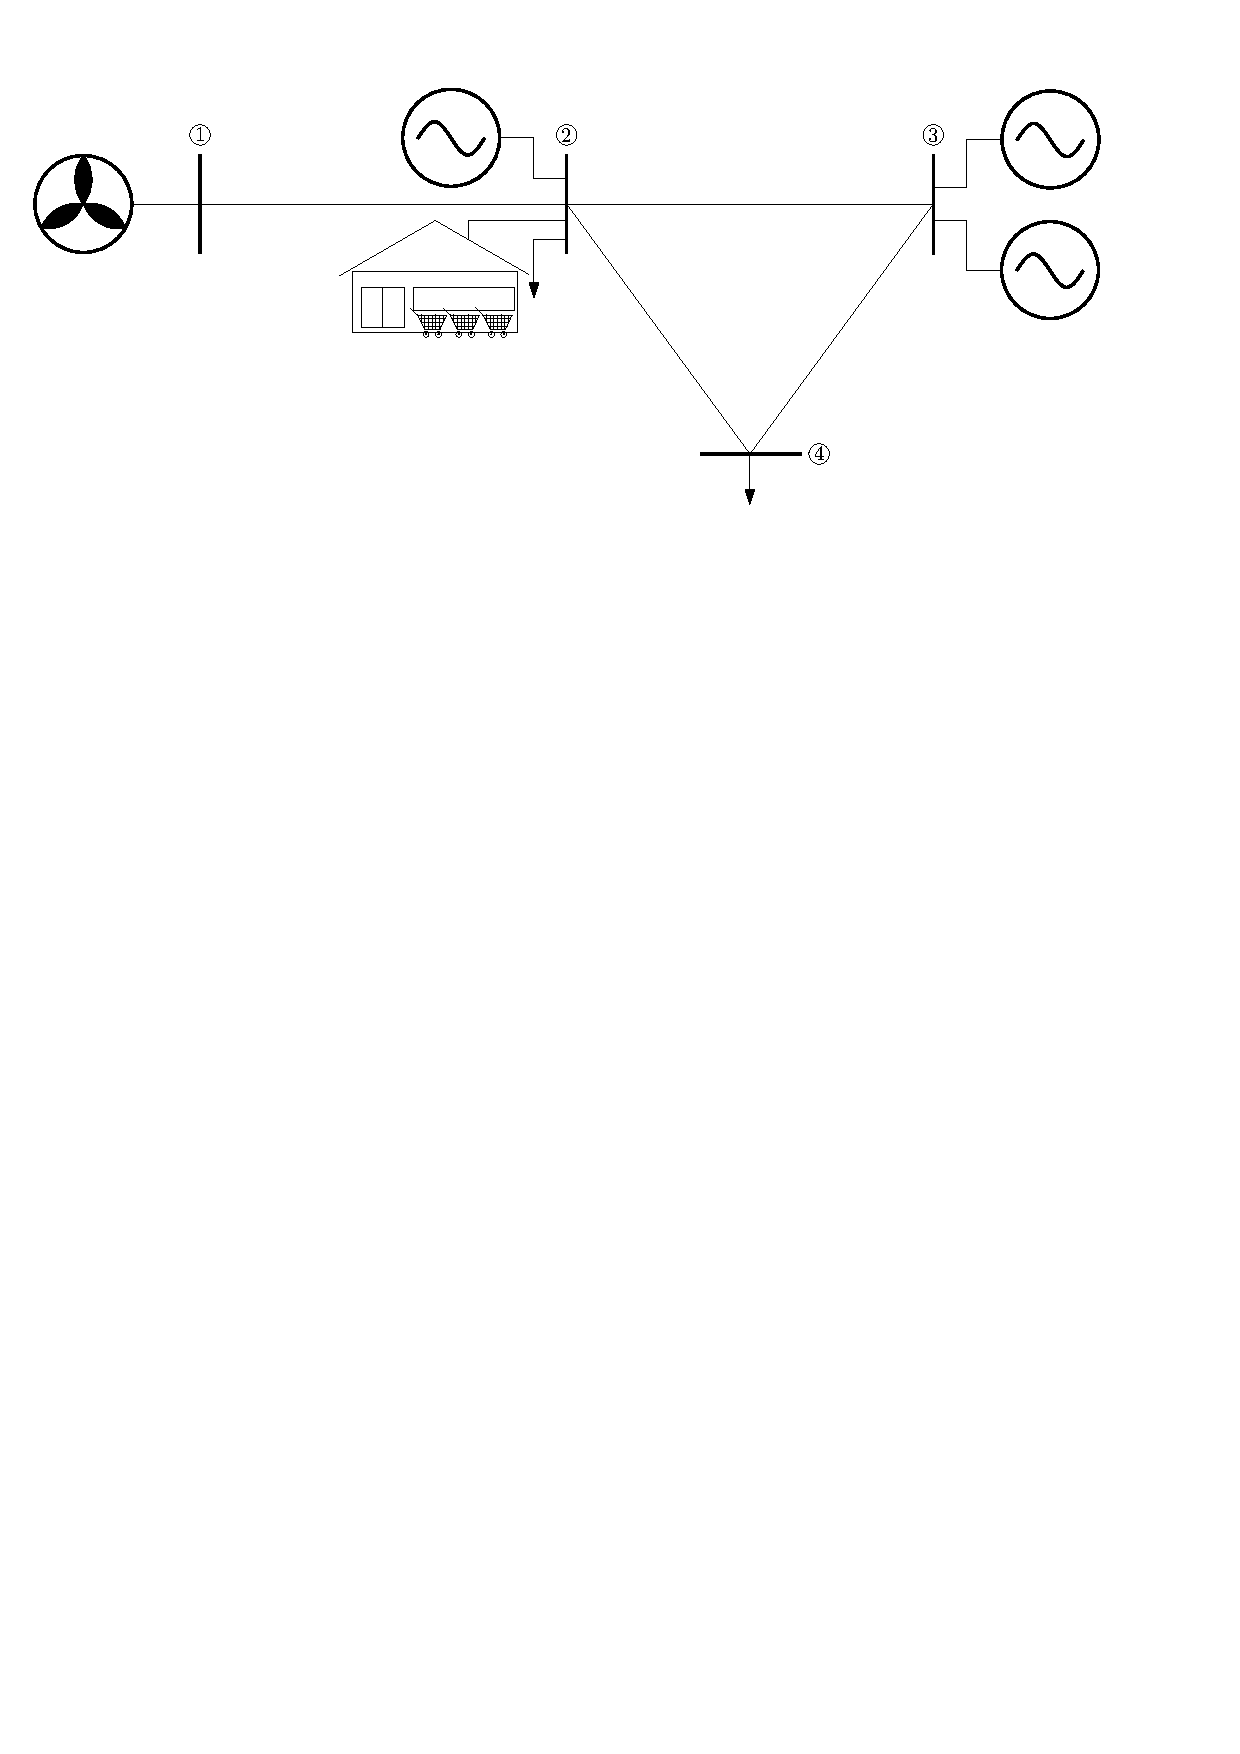
\includegraphics[scale=0.75]{images/SEVN/power_grid}
	\end{center}
\end{figure}

In der Realität kann ein Energieversorgungsnetz durch die Variation der Knotenzahl und die Vermaschung beliebig komplizierte
Form aufweisen. Bei der Umsetzung der gegebenen Situation im Programm.

\begin{figure}[h]
\caption{Klassendiagramm Modellkonstrukt}
	\label{klassendiagramm}
	\begin{center}
	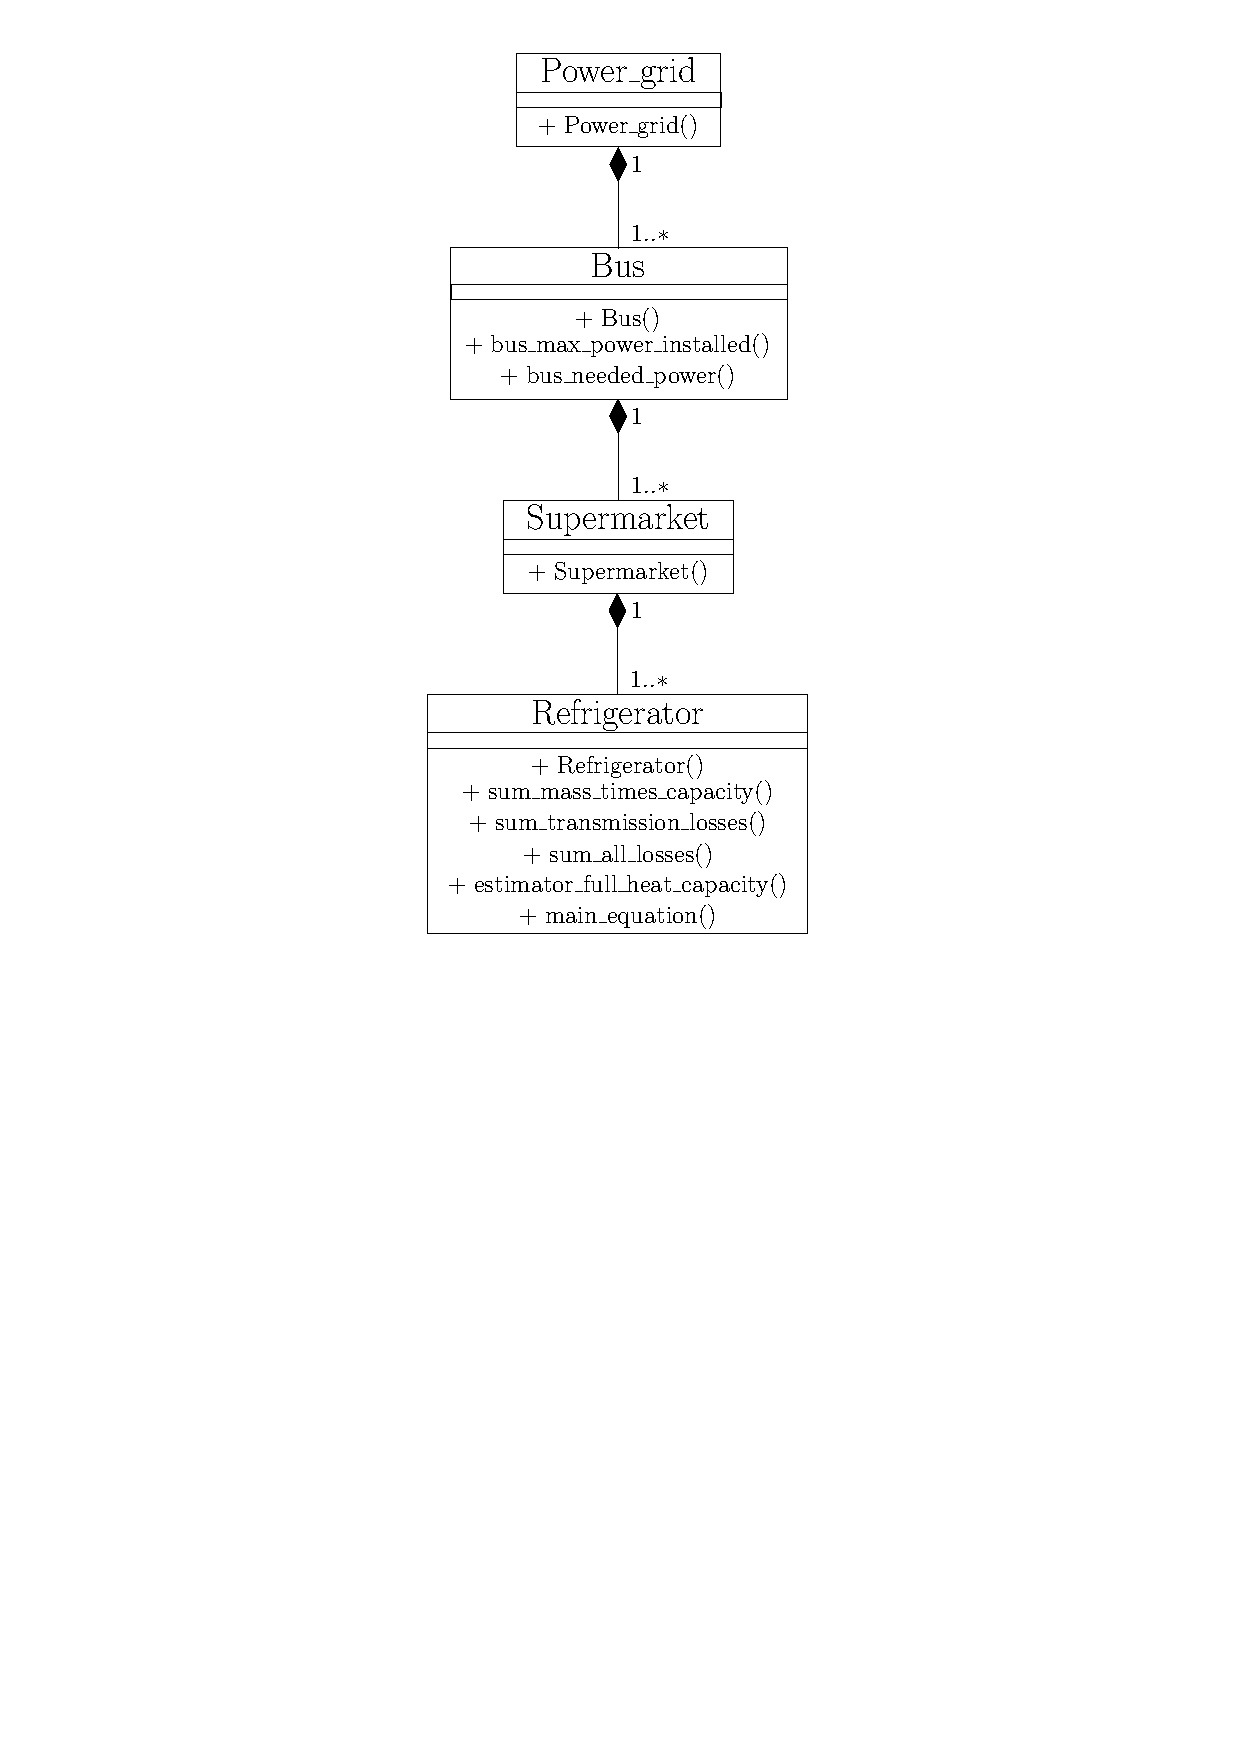
\includegraphics[scale=0.8]{images/Theorie_Super/class_diagramm}
	\end{center}
\end{figure}

Hier noch ein Zwischentext.

\begin{figure}[h]
\caption{Sequenzdiagramm Modellkonstrukt}
	\label{uml_sequence}
	\begin{center}
	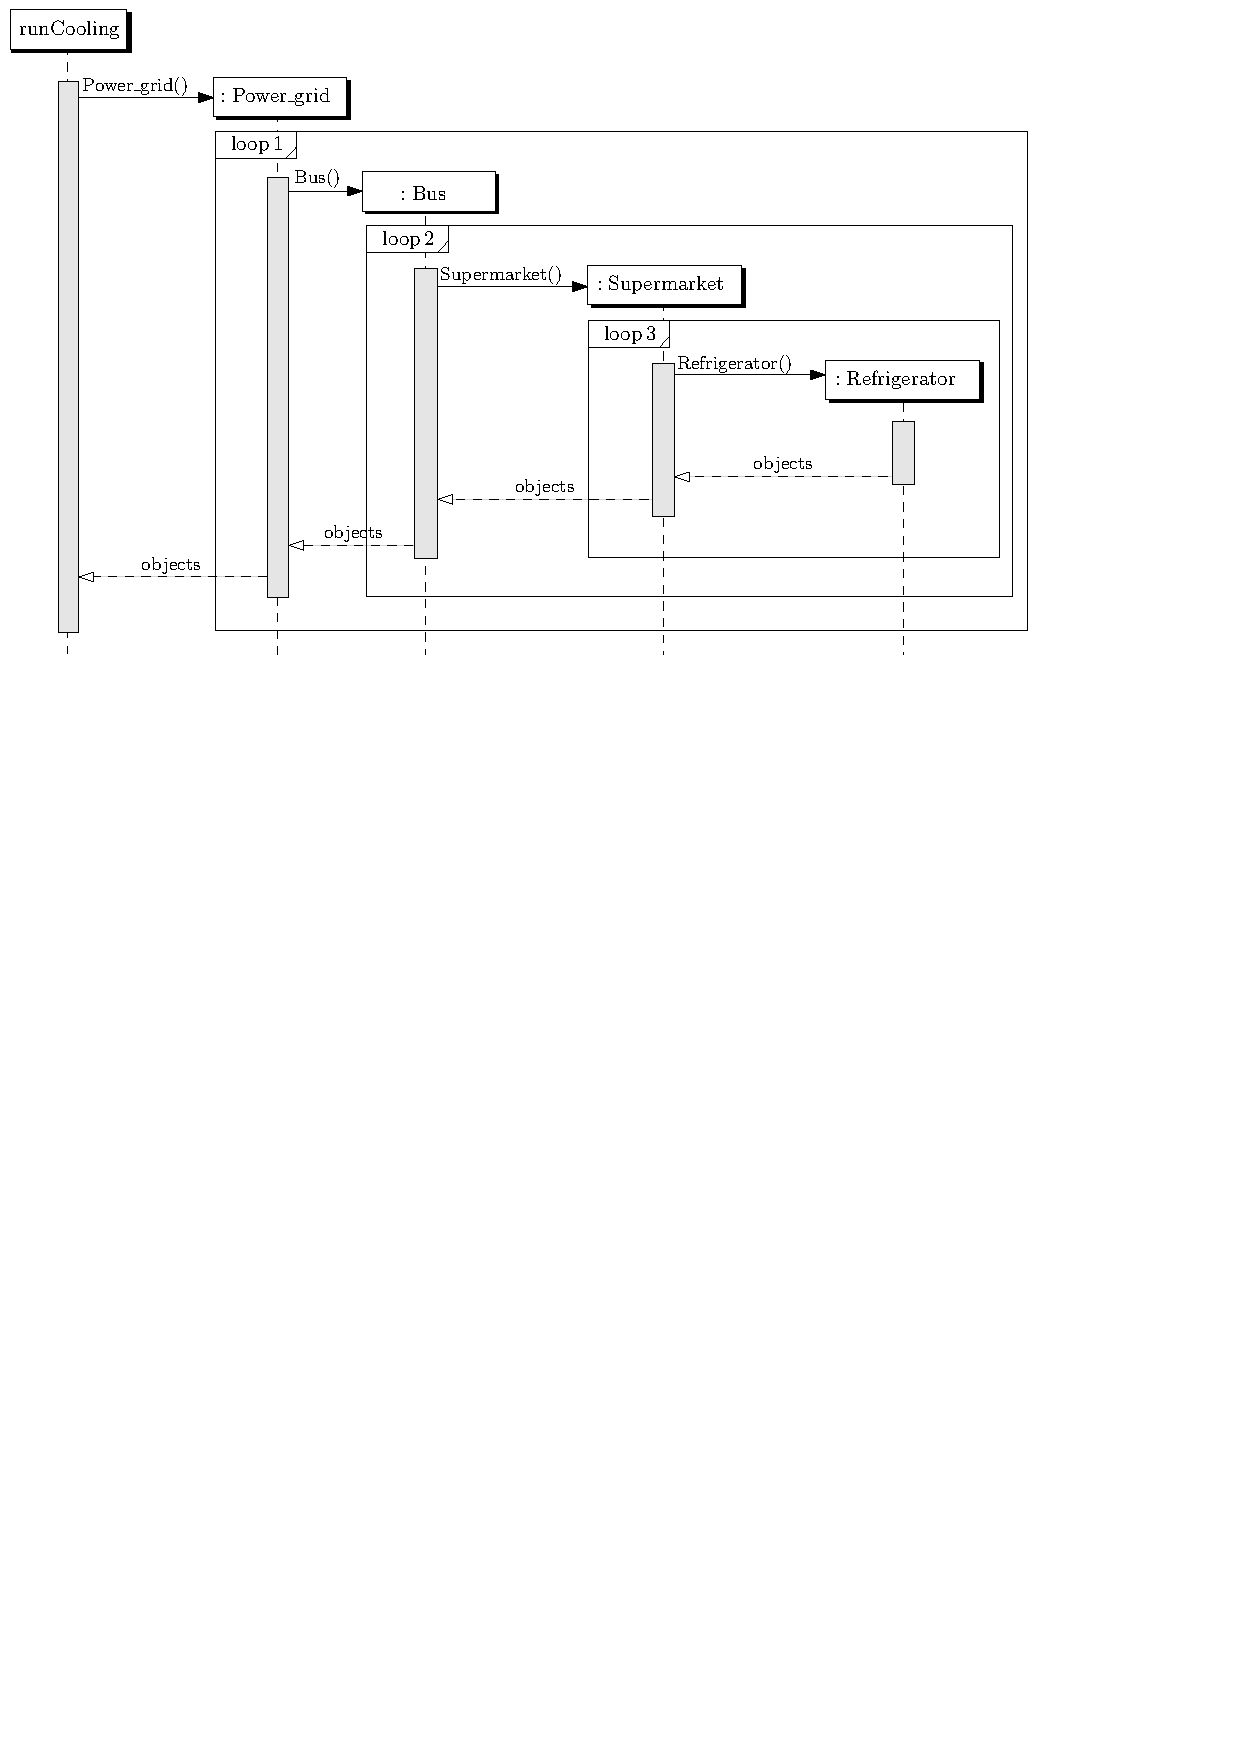
\includegraphics[scale=0.8]{images/Theorie_Super/sequence_one}
	\end{center}
\end{figure}

